\section{Question 4: Digit Recognition with CNN}

In this project, a handwritten digit recognition system running on ESP32-CAM has been developed using 5 different CNN models (SqueezeNet, EfficientNet, ResNet, MobileNet, ShuffleNet).

\subsection{Model Creation and Training}
The training process and creation stages of the models are detailed in the \texttt{Q4/digit\_recognition\_training.ipynb} Jupyter notebook. The general project structure and training steps are explained in \texttt{Q4/README.md}. The dataset used for training (shared with the YOLO task) is available at: \url{https://app.roboflow.com/ds/dYJXWYCHsE?key=3mqtC40lVJ}.

\subsection{Hardware Implementation and Inference}
The implementation in \texttt{ESP32\_CAM\_Digit\_Recognition.ino} integrates the TensorFlow Lite Micro library to perform on-device inference. The processing pipeline consists of the following stages:

\begin{enumerate}
    \item \textbf{Image Capture:} The ESP32 captures a QVGA (320x240) grayscale image.
    \item \textbf{Pre-processing:} The raw image undergoes several transformation steps to match the model's training data (MNIST):
    \begin{itemize}
        \item \textbf{Inversion:} The image colors are inverted (converting black-on-white text to white-on-black).
        \item \textbf{Noise Gate:} A threshold is applied (pixels < 50 set to 0) to remove background noise.
        \item \textbf{Contrast Stretching:} Pixel values are expanded to cover the full 0-255 dynamic range.
        \item \textbf{Resizing & Cropping:} The image is center-cropped and resized to 28x28 pixels using bilinear interpolation.
        \item \textbf{Quantization:} Pixels are normalized and converted to \texttt{int8} format suitable for the quantized model input.
    \end{itemize}
    \item \textbf{Inference:} The \texttt{MicroInterpreter} invokes the model using the pre-processed input tensor.
    \item \textbf{Output:} The probabilities for classes 0-9 are calculated from the output tensor, and the class with the highest probability is displayed via Serial and the Web Interface.
\end{enumerate}

\subsection{Results}
The visual results demonstrating the performance of the models are collected in the following folders:
\begin{itemize}
    \item \textbf{MobileNet Results:} \texttt{Q4/mobilenet}
    \item \textbf{ResNet Results:} \texttt{Q4/resnet}
\end{itemize}

\begin{figure}[H]
    \centering
    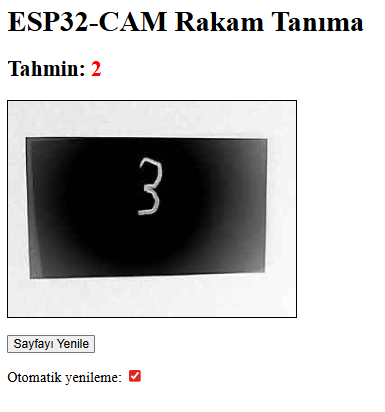
\includegraphics[width=0.7\textwidth]{../Q4/mobilenet/infer1.png}
    \caption{MobileNet Inference Result Example}
    \label{fig:q4_mobilenet}
\end{figure}

\begin{figure}[H]
    \centering
    
\includegraphics[width=0.7\textwidth]{../Q4/resnet/infer1.png}
    \caption{ResNet Inference Result Example}
    \label{fig:q4_resnet}
\end{figure}

\subsection{Encountered Errors}
During the deployment of \textbf{EfficientNet} and \textbf{ShuffleNet} models, the system failed to initialize the interpreter.

\textbf{Error Log:}
\begin{lstlisting}[basicstyle=\tiny, frame=single]
Didn't find op for builtin opcode 'SHAPE' version '1'. 
An older version of this builtin might be supported. 
Are you using an old TFLite binary with a newer model?
\end{lstlisting}

\textbf{Analysis:} This error indicates a version mismatch between the TensorFlow Lite Micro library used on the ESP32 (v1.0.0 by Tanaka Masayuki) and the operations required by these specific model architectures. The 'SHAPE' operation is likely introduced in a newer TensorFlow version or is implicitly required by the architecture of EfficientNet/ShuffleNet, but it is not implemented in the older `AllOpsResolver` or the specific library version available for the ESP32 environment.
